\section{Avaliação dos Modelos} \label{avaliacoes_dos_modelos}
Para avaliar o desempenho dos modelos de deteção de objetos, foi utilizada a matriz de confusão, e várias métricas padrão na área de Visão Computacional. As principais métricas consideradas foram:

\begin{itemize}
    \item \textbf{Precision (Precisão)}: Mede a proporção de predições corretas entre todas as predições positivas. Um valor elevado indica que o modelo comete poucos falsos positivos.
    
    \item \textbf{Recall (Revocação)}: Mede a proporção de objetos verdadeiros que foram corretamente detetados. Um valor elevado indica que o modelo falha poucas vezes as deteções.
    
    \item \textbf{mAP@50 (Mean Average Precision a 50\% IoU)}: É a média da precisão ao longo de todas as classes, e a mais comum em benchmarks. Deve estar o mais próximo possível de 1.
    
    \item \textbf{mAP@50-95}: É a média da mAP considerando múltiplos limiares de IoU entre 50\% e 95\%, com incrementos de 5\%. Esta métrica é mais exigente e fornece uma avaliação mais abrangente.
    
    \item \textbf{Perdas (Losses)}: Foram monitorizadas as perdas de \textit{box\_loss}, \textit{cls\_loss} e \textit{dfl\_loss} durante o treino e validação. Estas perdas indicam o erro cometido na regressão da caixa delimitadora, na classificação e na distribuição espacial das previsões, respetivamente.
\end{itemize}

%
% Modelos PokeMMO
%
\subsection{Modelos do PokeMMO}
Foram treinados dois modelos com os mesmos parâmetros. Ambos foram treinados durante 100 épocas. No entanto, um dos modelos foi treinado com o \textit{YOLOv8m} e o outro com o \textit{YOLOv8x}, sendo que este último é, teoricamente, uma versão superior à versão \textit{m}. Como tal, requer mais tempo de treino e maior capacidade computacional. Assim, será realizada uma avaliação onde se irá comparar os dois modelos iniciais, de forma a determinar se o tempo e os recursos investidos no treino da versão \textit{x} são justificáveis e se faz sentido optar por esta versão nos treinos de modelos futuros.

\begin{figure}[h]
    \centering
    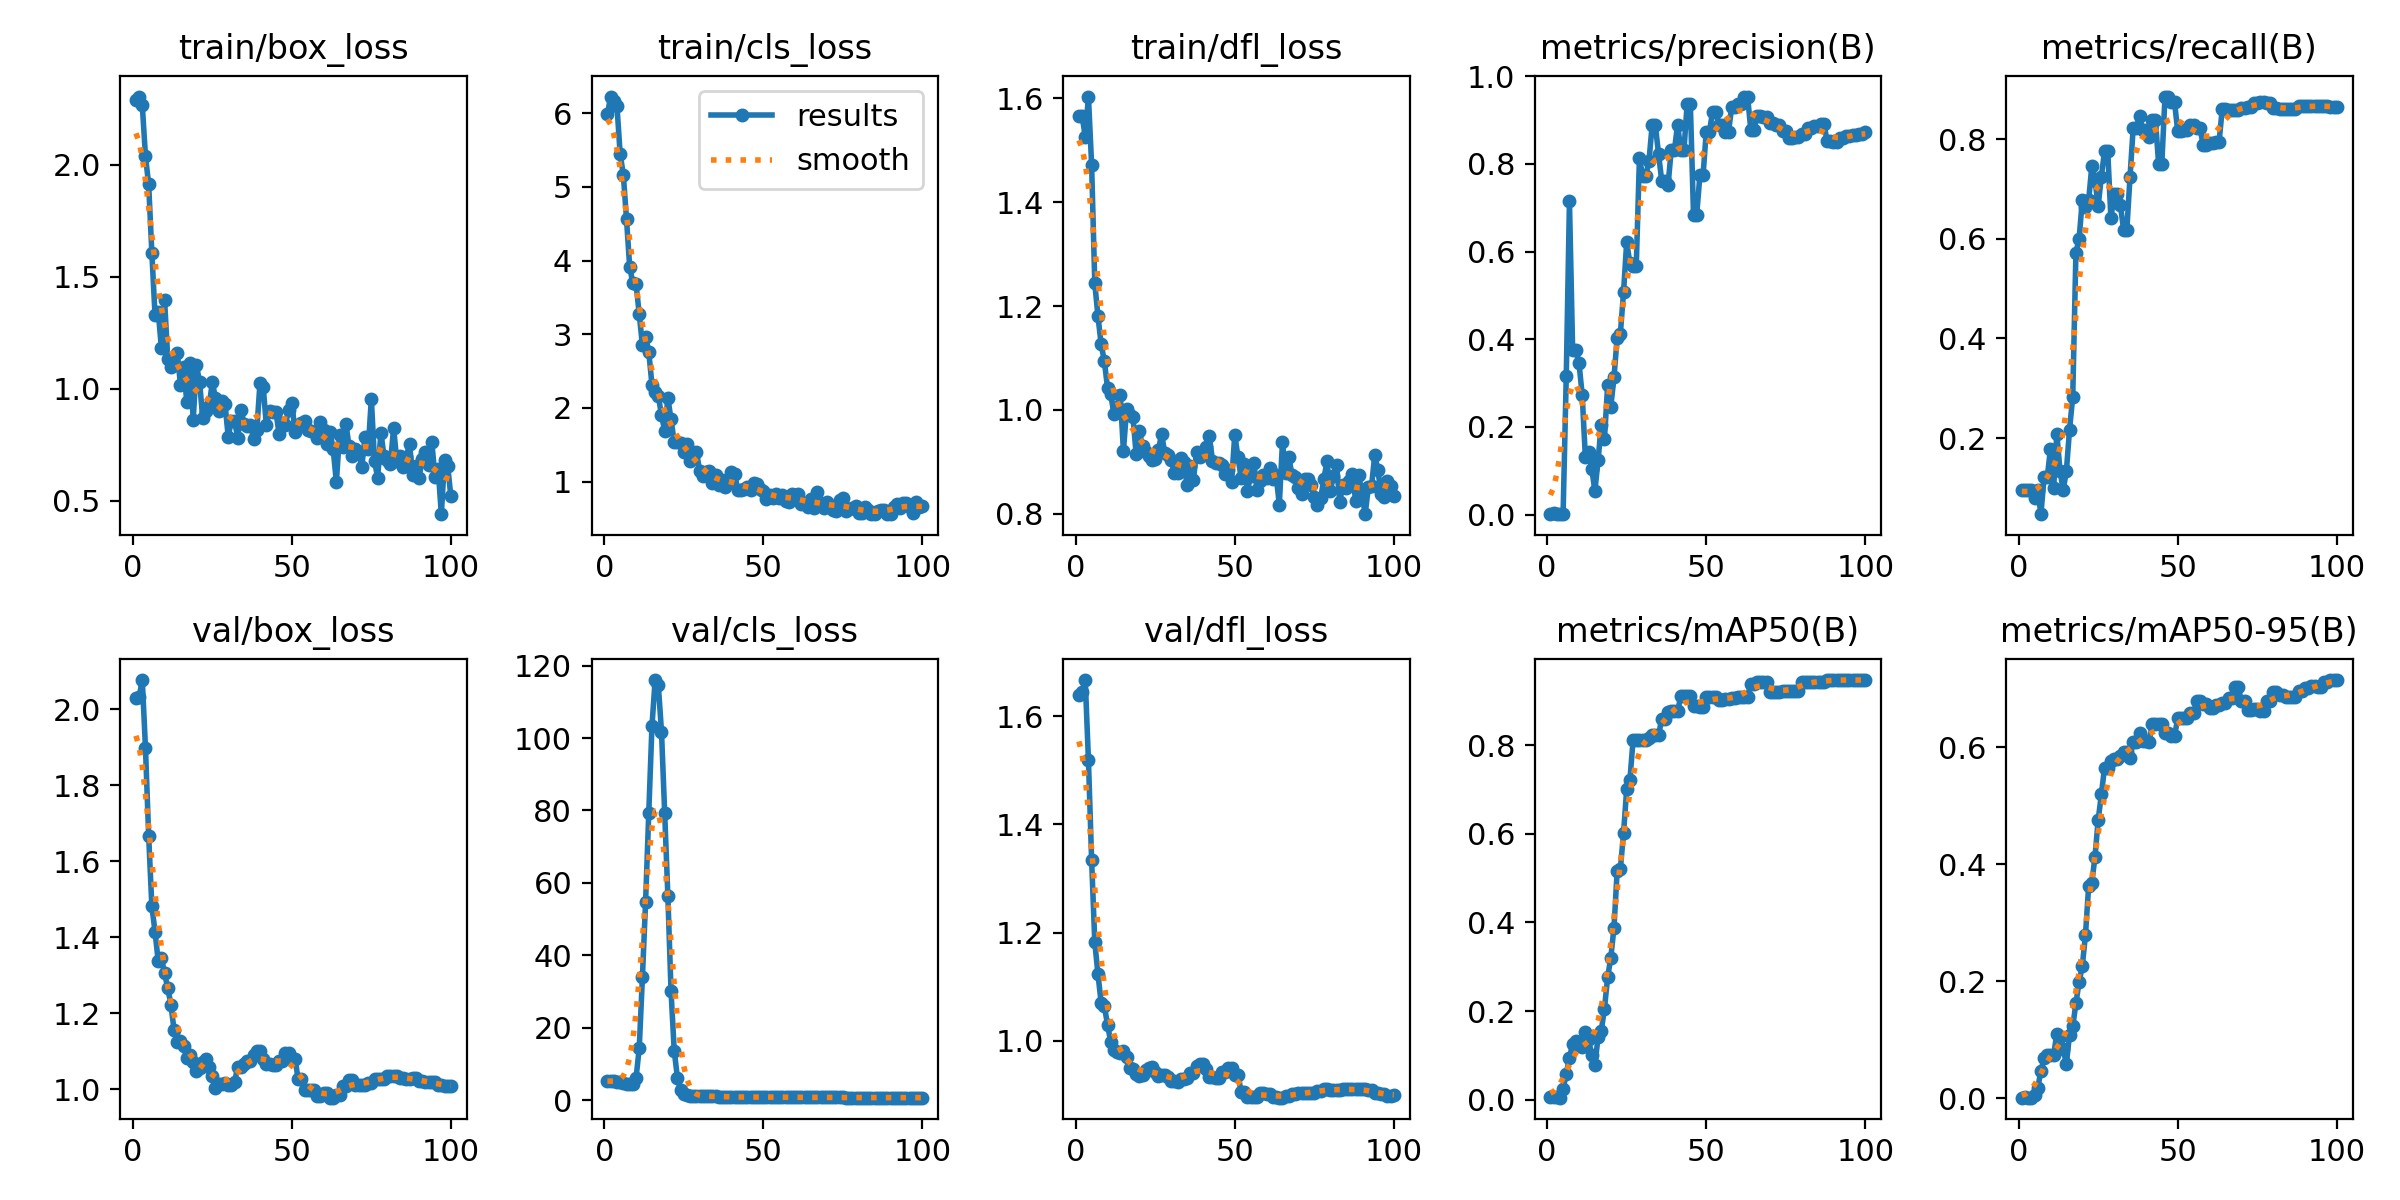
\includegraphics[width=0.7\textwidth]{imagens/results_modelom.png}
    \caption{Gráficos de desempenho do primeiro modelo criado para o PokeMMO (YOLOv8m).}
    \label{fig:results_modelom}
\end{figure}

\begin{figure}[h]
    \centering
    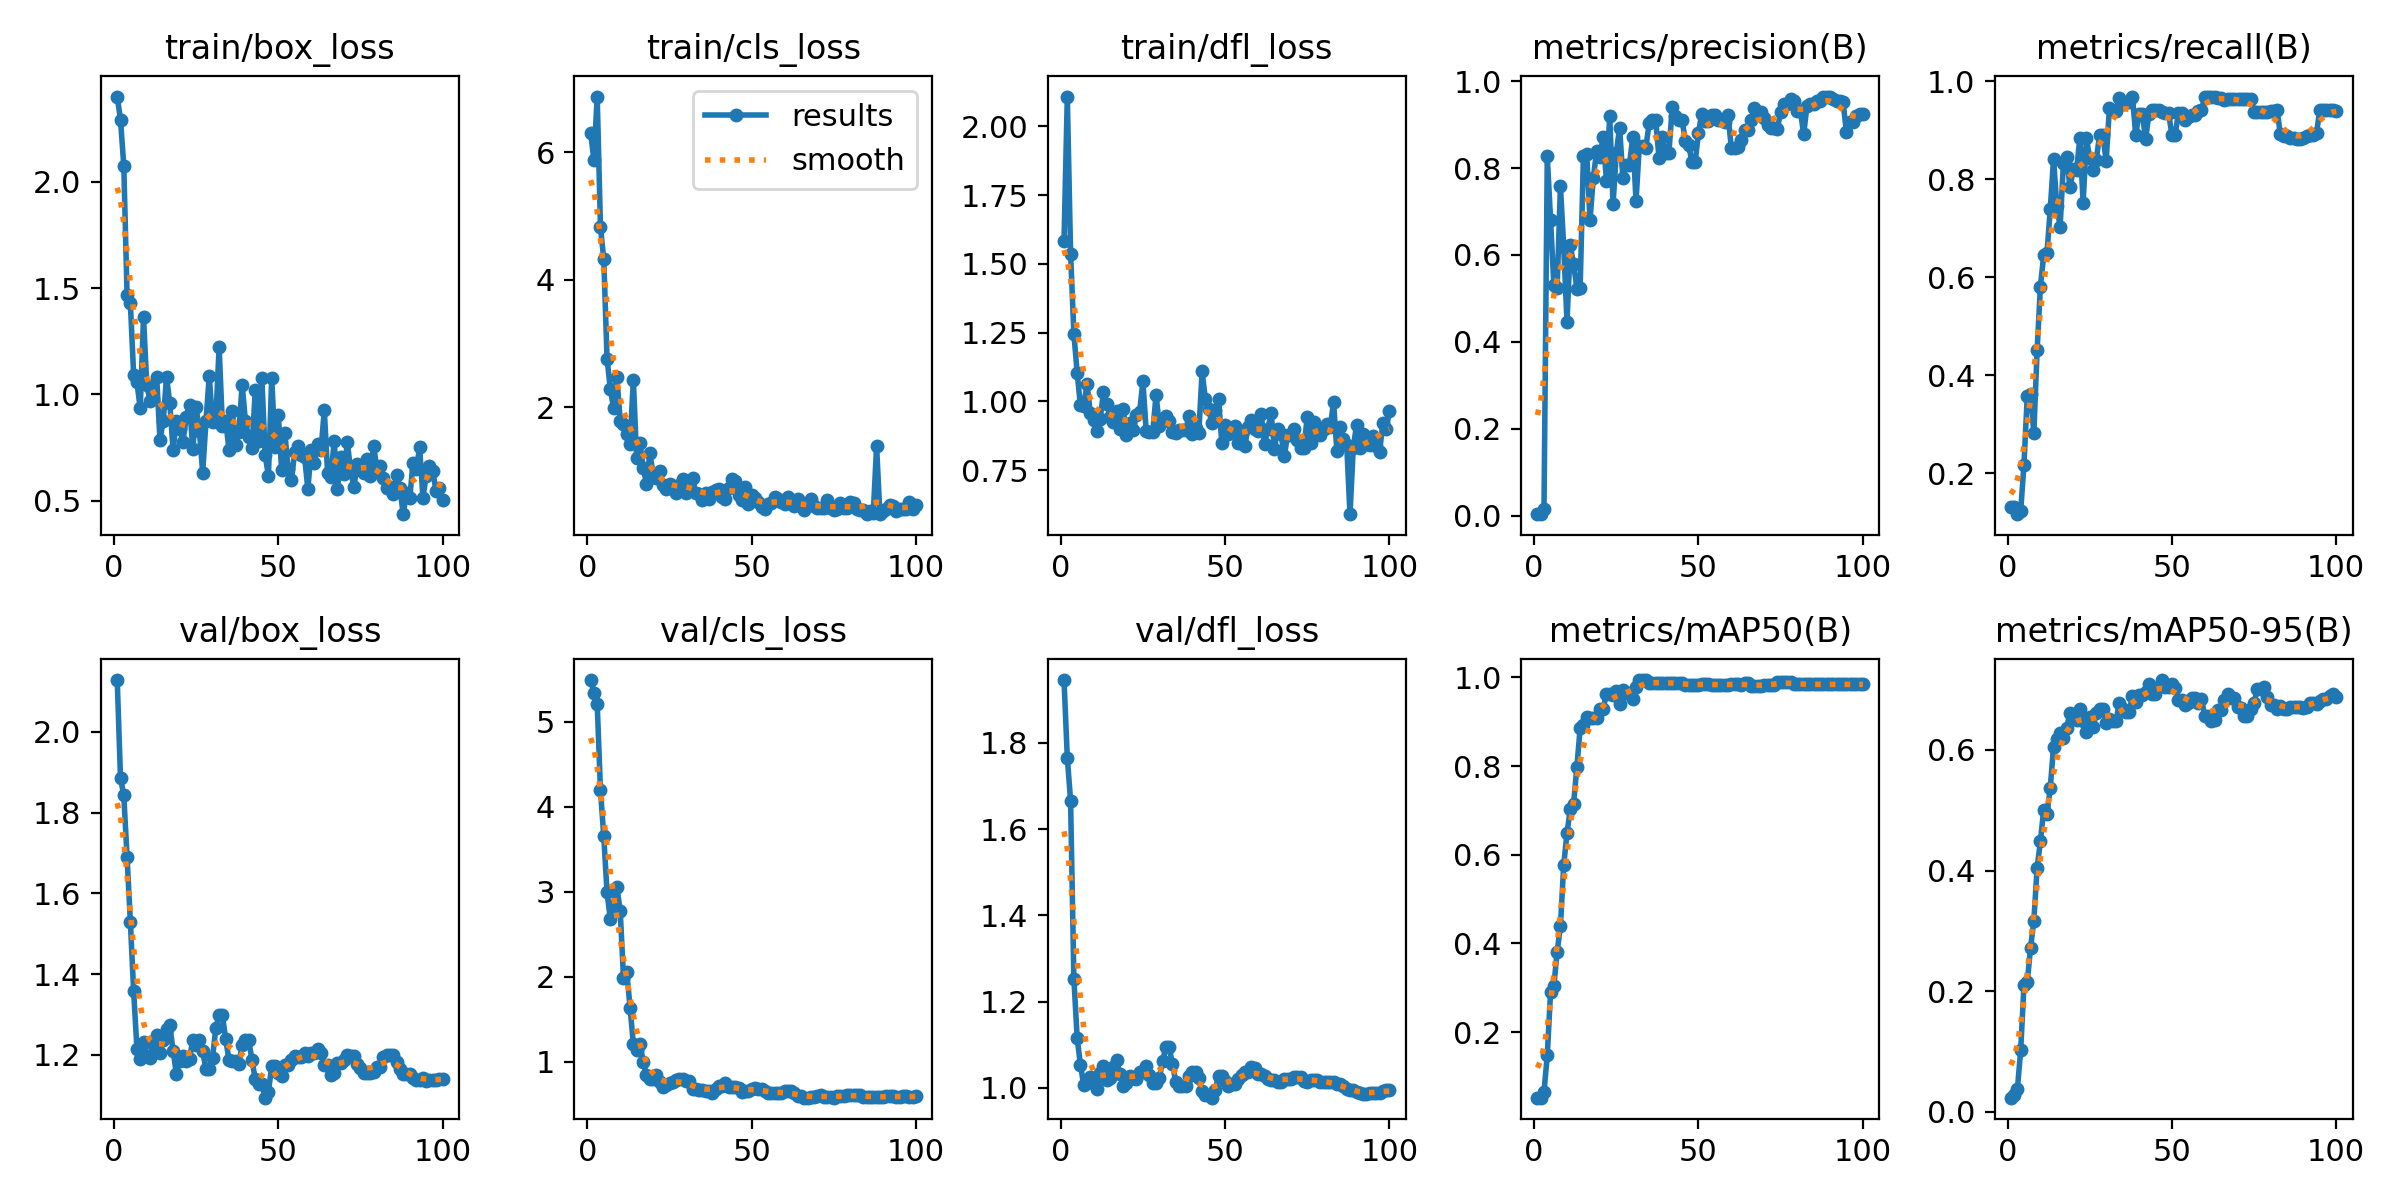
\includegraphics[width=0.7\textwidth]{imagens/results_modelox.png}
    \caption{Gráficos de desempenho do segundo modelo criado para o PokeMMO(YOLOv8x).}
    \label{fig:results_modelox}
\end{figure}

A parir dos gráficos de desempenho de cada modelo nas figuras \ref{fig:results_modelom} e \ref{fig:results_modelox} observa-se que:

\begin{itemize}
    \item As métricas de \textbf{precision} e \textbf{recall} estabilizaram acima dos 90\% em ambos os modelos, mas é possível visualizar que no modelo \textit{x} a linha não oscilou tanto, para além de se ter estabilizando mais cedo acima dos 90\%.
    
    \item O \textbf{mAP@50} aproxima-se de 1.0, o que indica uma excelente performance nas deteções, mais uma vez é possível detetar algumas oscilações no modelo \textit{m}, e uma aproximação de 1.0 mais cedo no modelo \textit{x}.
    
    \item O \textbf{mAP@50-95} estabilizou por volta de 0.7, o que demonstra boa generalização mesmo em critérios mais exigentes.
    
    \item As \textbf{perdas de validação} diminuíram progressivamente e estabilizaram, sem sinais evidentes de overfitting.
\end{itemize}

A partir das métricas analisadas, é possível concluir que o modelo \textit{YOLOv8x} apresentou um desempenho ligeiramente superior ao modelo \textit{YOLOv8m}. Isso é reforçado não apenas pelas curvas mais estáveis e pela convergência mais rápida nas métricas principais, mas também pelas matrizes de confusão, onde se observa que o modelo \textit{m} cometeu mais erros de classificação do que o modelo \textit{x}.

\begin{figure}[h]
    \centering
    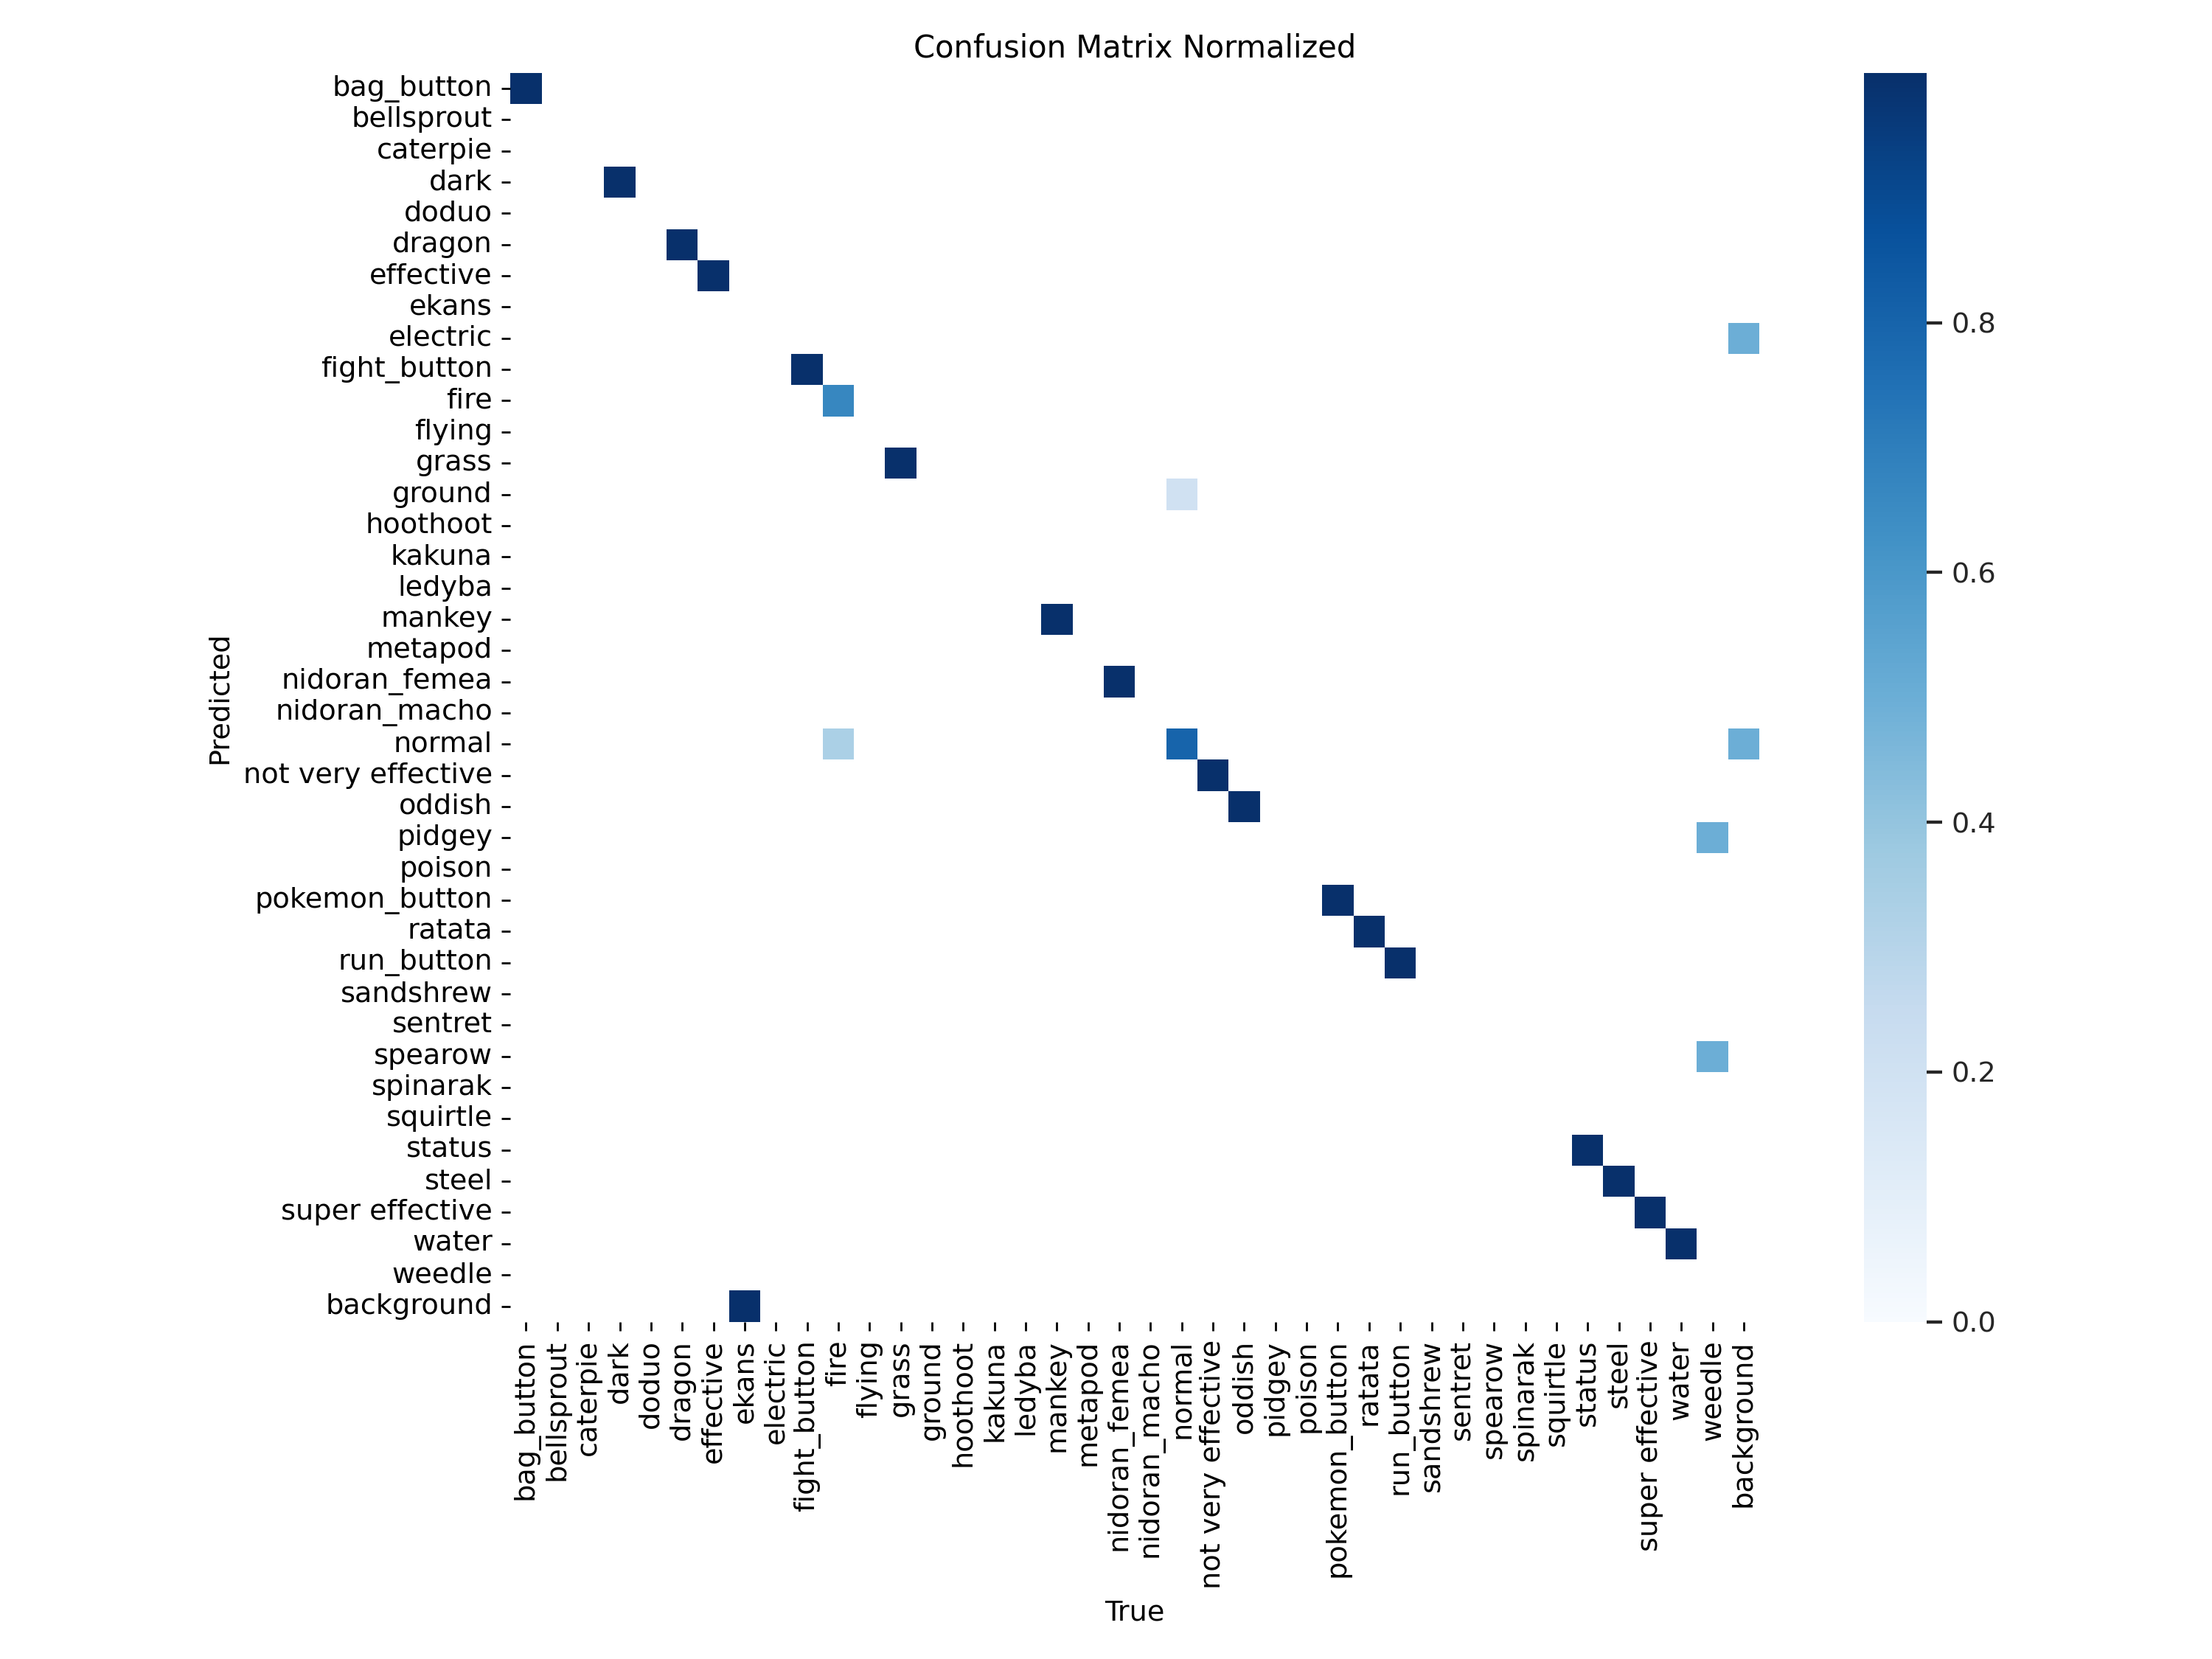
\includegraphics[width=0.65\textwidth]{imagens/confusion_matrix_normalized_modelom.png}
    \caption{Matriz de confusão do primeiro modelo criado para o PokeMMO (YOLOv8m).}
    \label{fig:confusion_matrix_modelom}
\end{figure}

\begin{figure}[h]
    \centering
    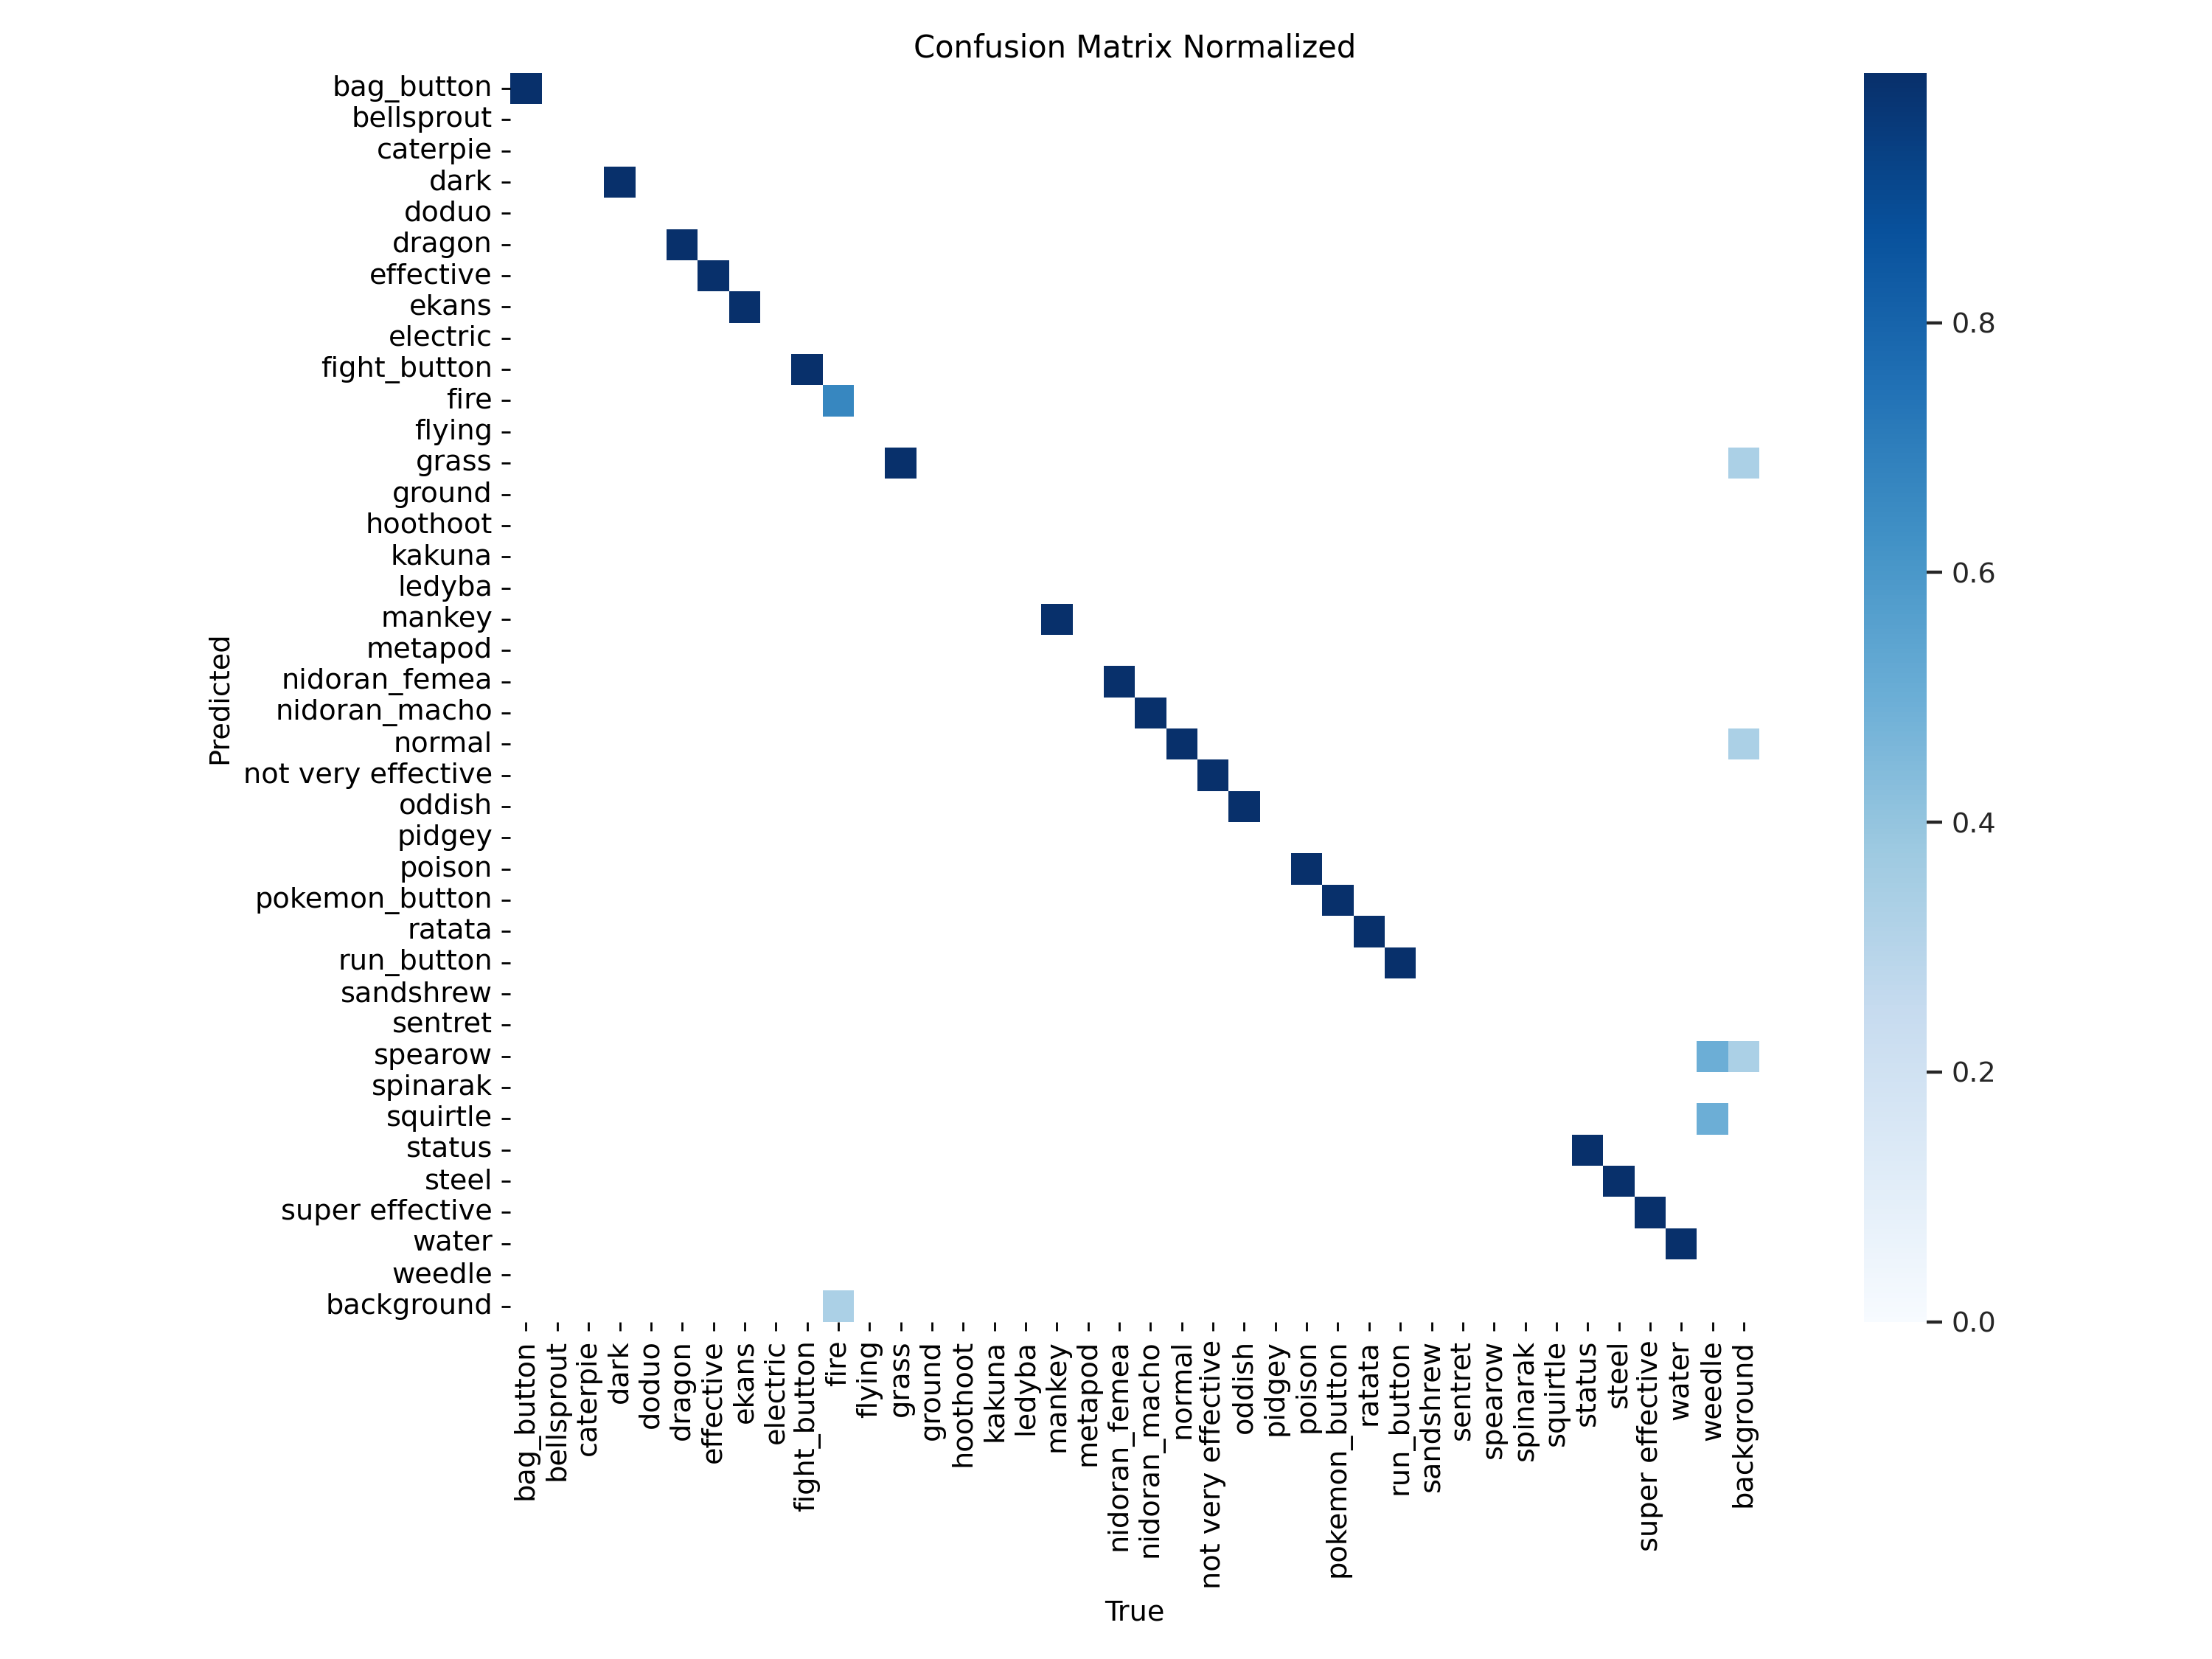
\includegraphics[width=0.65\textwidth]{imagens/confusion_matrix_normalized_modelox.png}
    \caption{Matriz de confusão do segundo modelo criado para o PokeMMO (YOLOv8x).}
    \label{fig:confusion_matrix_modelox}
\end{figure}

Apesar das melhorias não serem extremamente significativas, o modelo \textit{YOLOv8x} demonstrou maior robustez, especialmente na redução de falsos positivos. Por essa razão, decidiu-se utilizá-lo como base para os modelos treinados nas etapas seguintes.



%
% Modelos PokemonHeartGold
%
\subsection{Modelos do Pokémon HeartGold}
Para o jogo Pokémon HeartGold foram treinados vários modelos diferentes, onde a cada modelo era um incremento do modelo anterior, onde eram adicionadas novas classes para identificar objetos diferentes no ecrã. O primeiro modelo foi treinado com um número reduzido de classes, enquanto que o último modelo foi treinado com um conjunto mais completo de classes. Ambos os modelos utilizaram o mesmo modelo (\textit{YOLOv8x}) e foram treinados com 100 épocas, sendo a principal diferença entre os modelos a complexidade e diversidade dos dados de treino, com o último modelo a incluir técnicas de \textit{data augmentation} para melhorar a generalização.

Deste modo, será realizada uma análise comparativa entre os dois modelos, mesmo reconhecendo que os conjuntos de dados e os objetivos de cada um não são exatamente equivalentes. O objetivo desta comparação é perceber se, com o aumento da complexidade, se houve uma evolução significativa na capacidade de deteção e desempenho geral do sistema.

\begin{figure}[h]
    \centering
    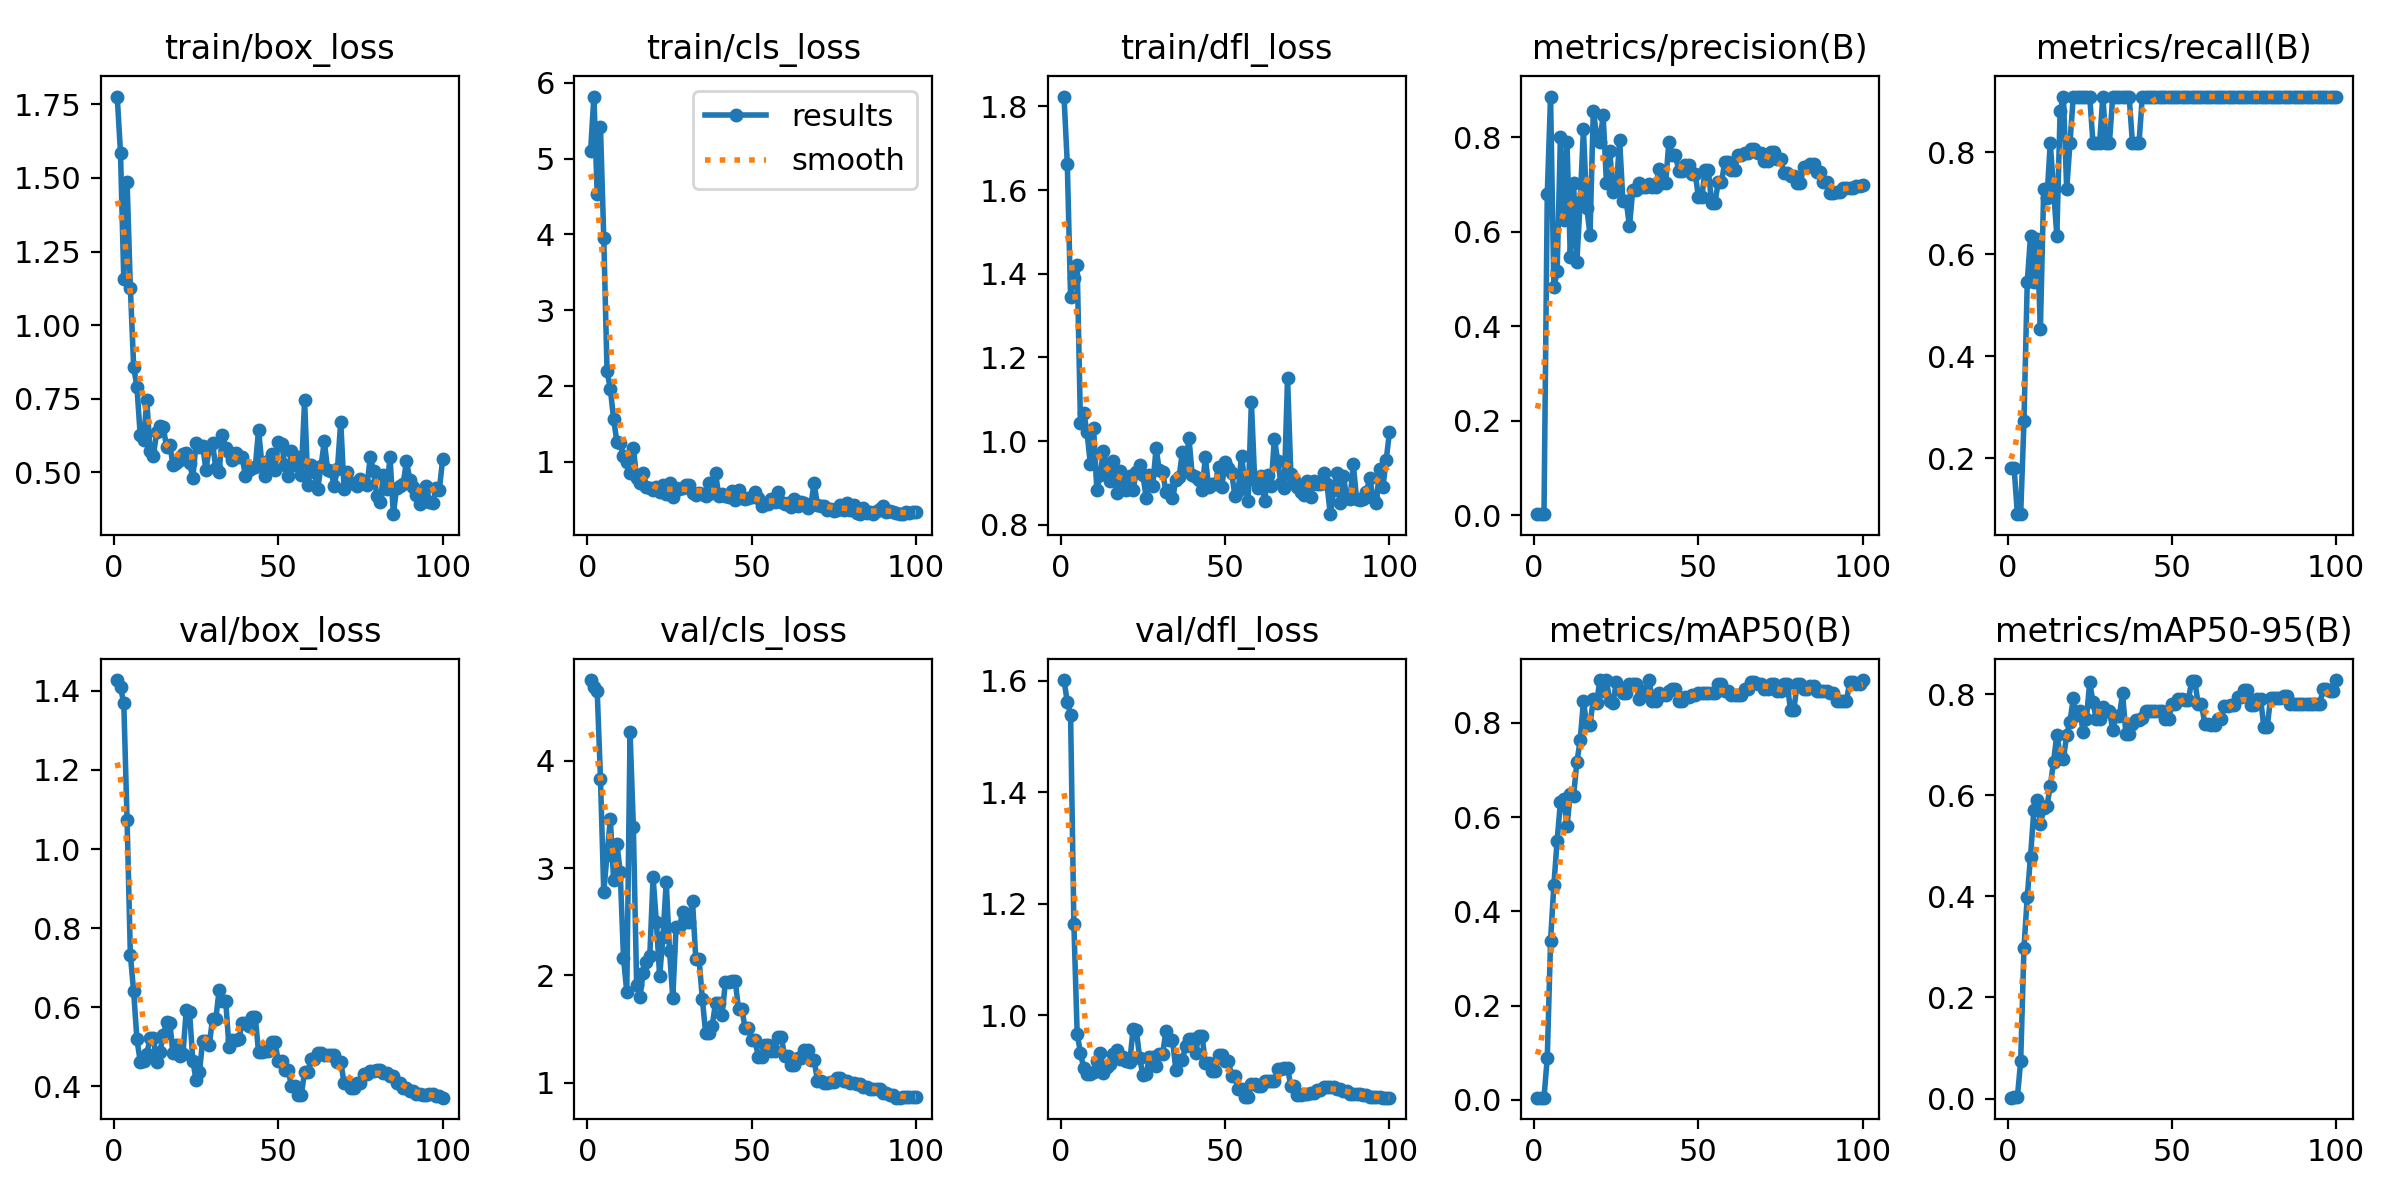
\includegraphics[width=0.80\textwidth]{imagens/results_primeiro_modelo.png}
    \caption{Gráficos de desempenho do primeiro modelo criado para o Pokémon HeartGold.}
    \label{fig:results_primeiro_modelo}
\end{figure}

\begin{figure}[h]
    \centering
    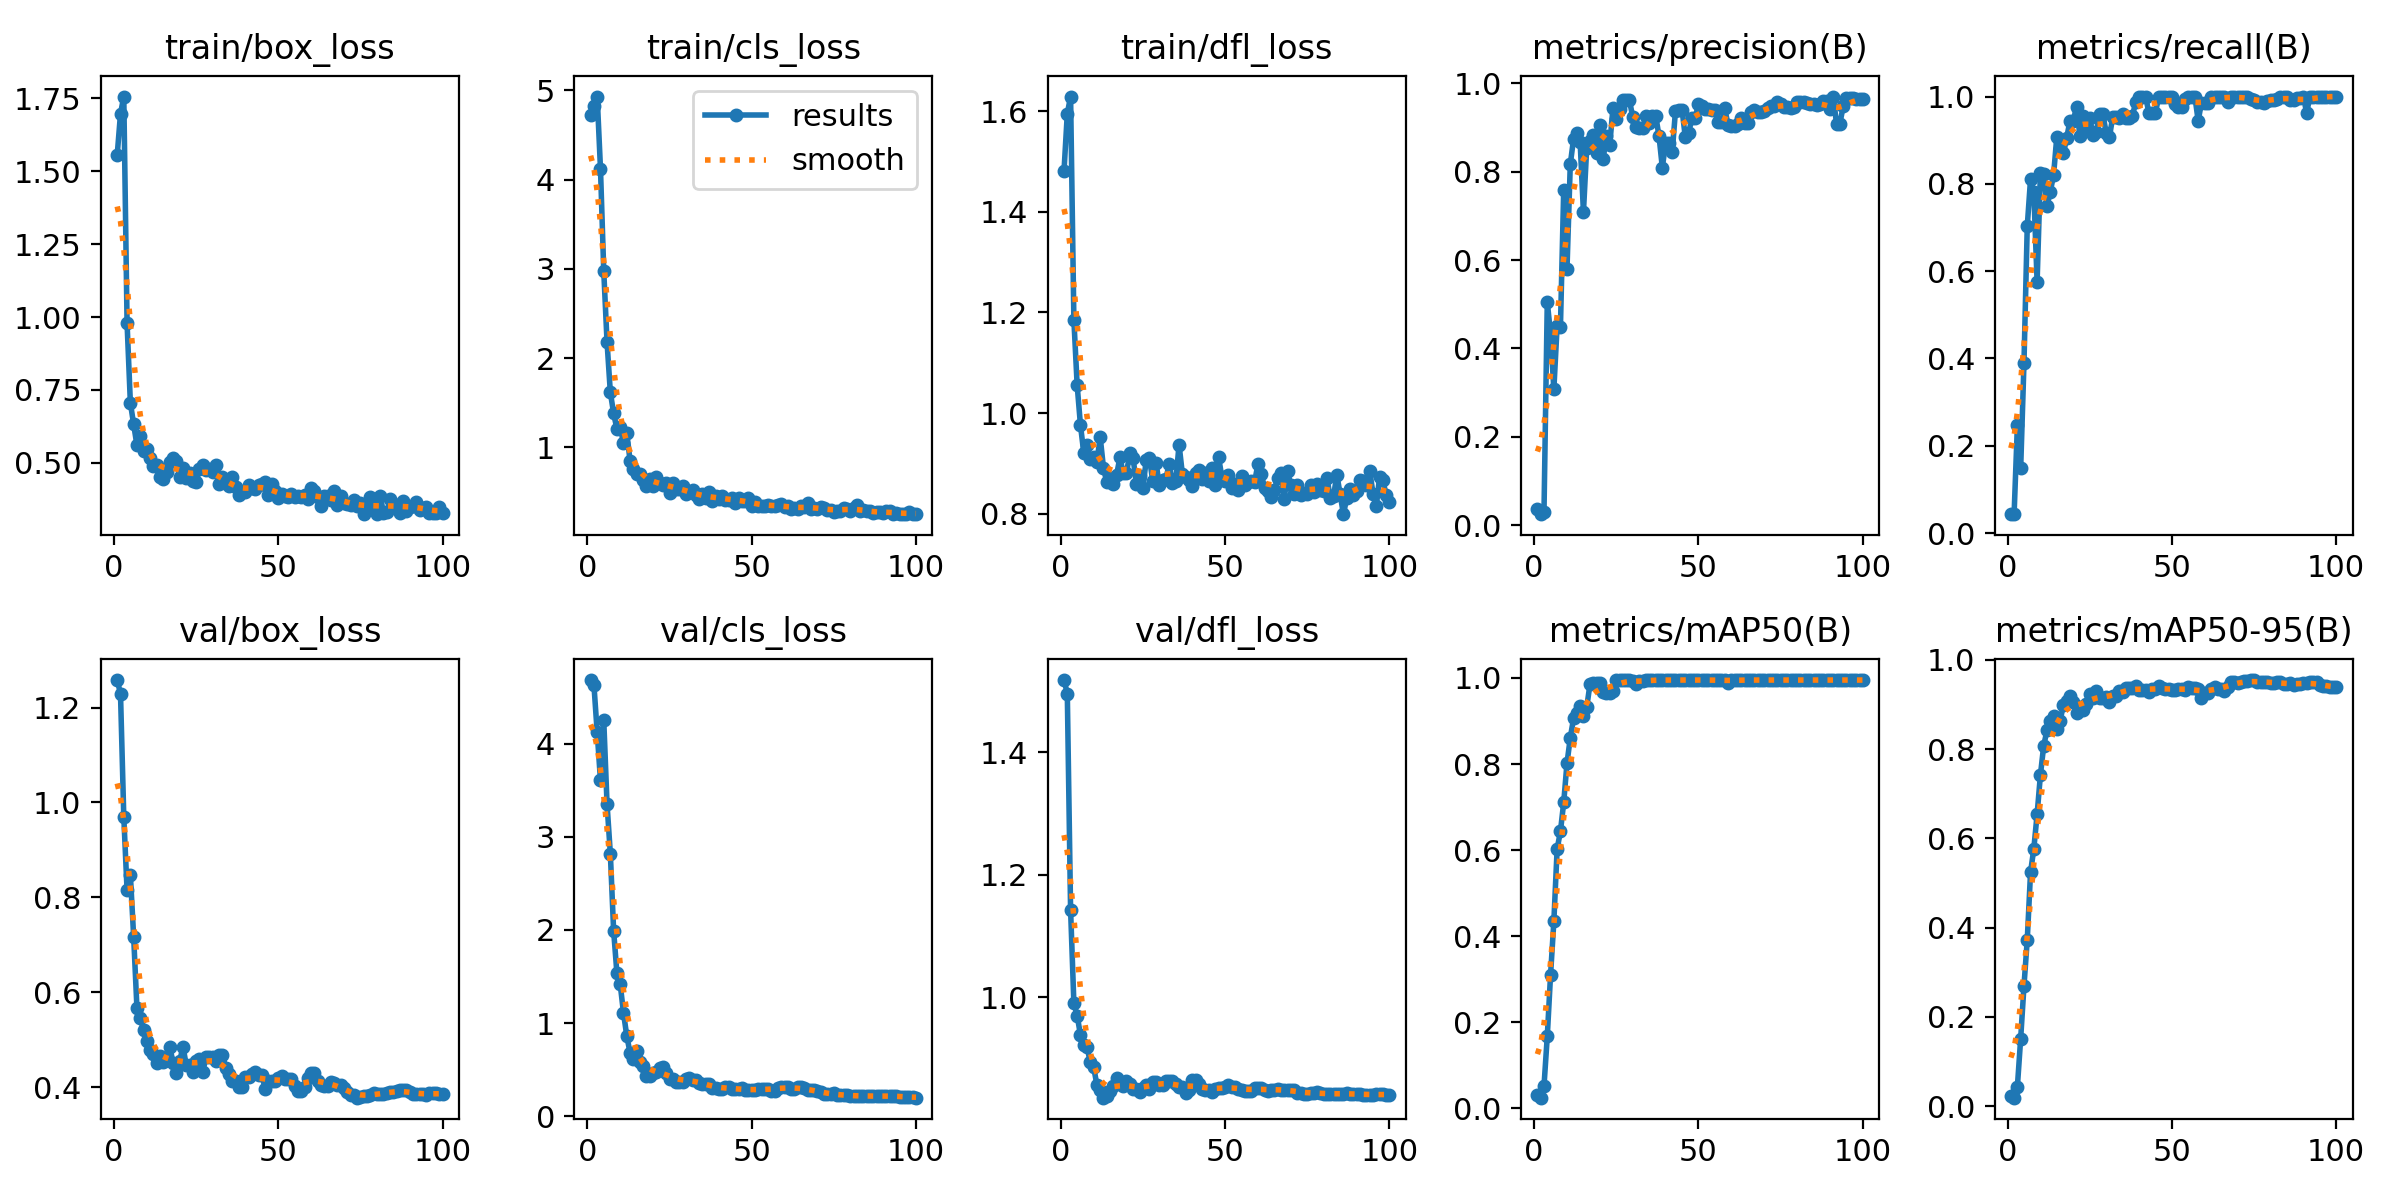
\includegraphics[width=0.80\textwidth]{imagens/results_ultimo_modelo.png}
    \caption{Gráficos de desempenho do segundo (e último) modelo criado para o Pokémon HeartGold.}
    \label{fig:results_ultimo_modelo}
\end{figure}

A partir das figuras \ref{fig:results_primeiro_modelo} e \ref{fig:results_ultimo_modelo} observa-se que:

\begin{itemize}
    \item As métricas de \textbf{precision} e \textbf{recall} estabilizaram-se mais rapidamente no último modelo, com valores superiores a 95\%, enquanto que no primeiro modelo estes valores oscilaram mais nas primeiras épocas.
    
    \item O \textbf{mAP@50} aproxima-se de 1.0 em ambos os modelos, no entanto, a convergência para esse valor é visivelmente mais rápida e estável no segundo modelo.
    
    \item O \textbf{mAP@50-95} é significativamente superior no segundo modelo, aproximando-se de 0.95, o que indica uma generalização muito mais eficaz, mesmo com critérios mais exigentes.
    
    \item As \textbf{perdas de treino e validação} diminuíram de forma mais acentuada no segundo modelo, mantendo-se baixas e estáveis ao longo do treino, sugerindo uma boa adaptação sem sinais de \textit{overfitting}.
\end{itemize}

% Matriz de confusão

Ao analisar as matrizes de confusão normalizadas das Figuras \ref{fig:confusion_matrix_primeiro_modelo} e \ref{fig:confusion_matrix_ultimmo_modelo}, observa-se um comportamento inesperado no segundo modelo (modelo final). Este apresenta uma matriz de confusão praticamente perfeita, sem registo de erros de classificação, o que, teoricamente, indicaria uma taxa de acerto de 100\% em todas as classes.

No entanto, na prática, durante os testes com o modelo em produção, foi possível verificar que este ainda comete alguns erros ocasionais, embora em pequena quantidade. Essa discrepância entre o desempenho observado na validação e o comportamento real pode estar relacionada com vários fatores, sendo os mais prováveis:

\begin{itemize}
    \item \textbf{Pouca diversidade no  conjunto de validação}: O conjunto de validação utilizado pode não representar de forma completa a variedade de situações e imagens reais enfrentadas pelo modelo em produção. Isso pode levar a uma avaliação artificialmente otimista.
    
    \item \textbf{Overfitting parcial ao conjunto de validação}: Mesmo que o modelo não mostre sinais evidentes de \textit{overfitting} nas métricas gerais, pode ter aprendido padrões muito específicos ao conjunto de validação, o que explicaria a performance quase perfeita nas métricas internas, mas um desempenho inferior em imagens não vistas anteriormente.
    
    \item \textbf{Imprecisão na anotação dos dados de produção}: As falhas observadas podem também estar relacionadas com diferenças nas condições visuais das imagens reais (luminosidade, resolução, sobreposição de elementos), que não estão refletidas nos dados de treino ou validação.
\end{itemize}

\begin{figure}[!h]
    \centering
    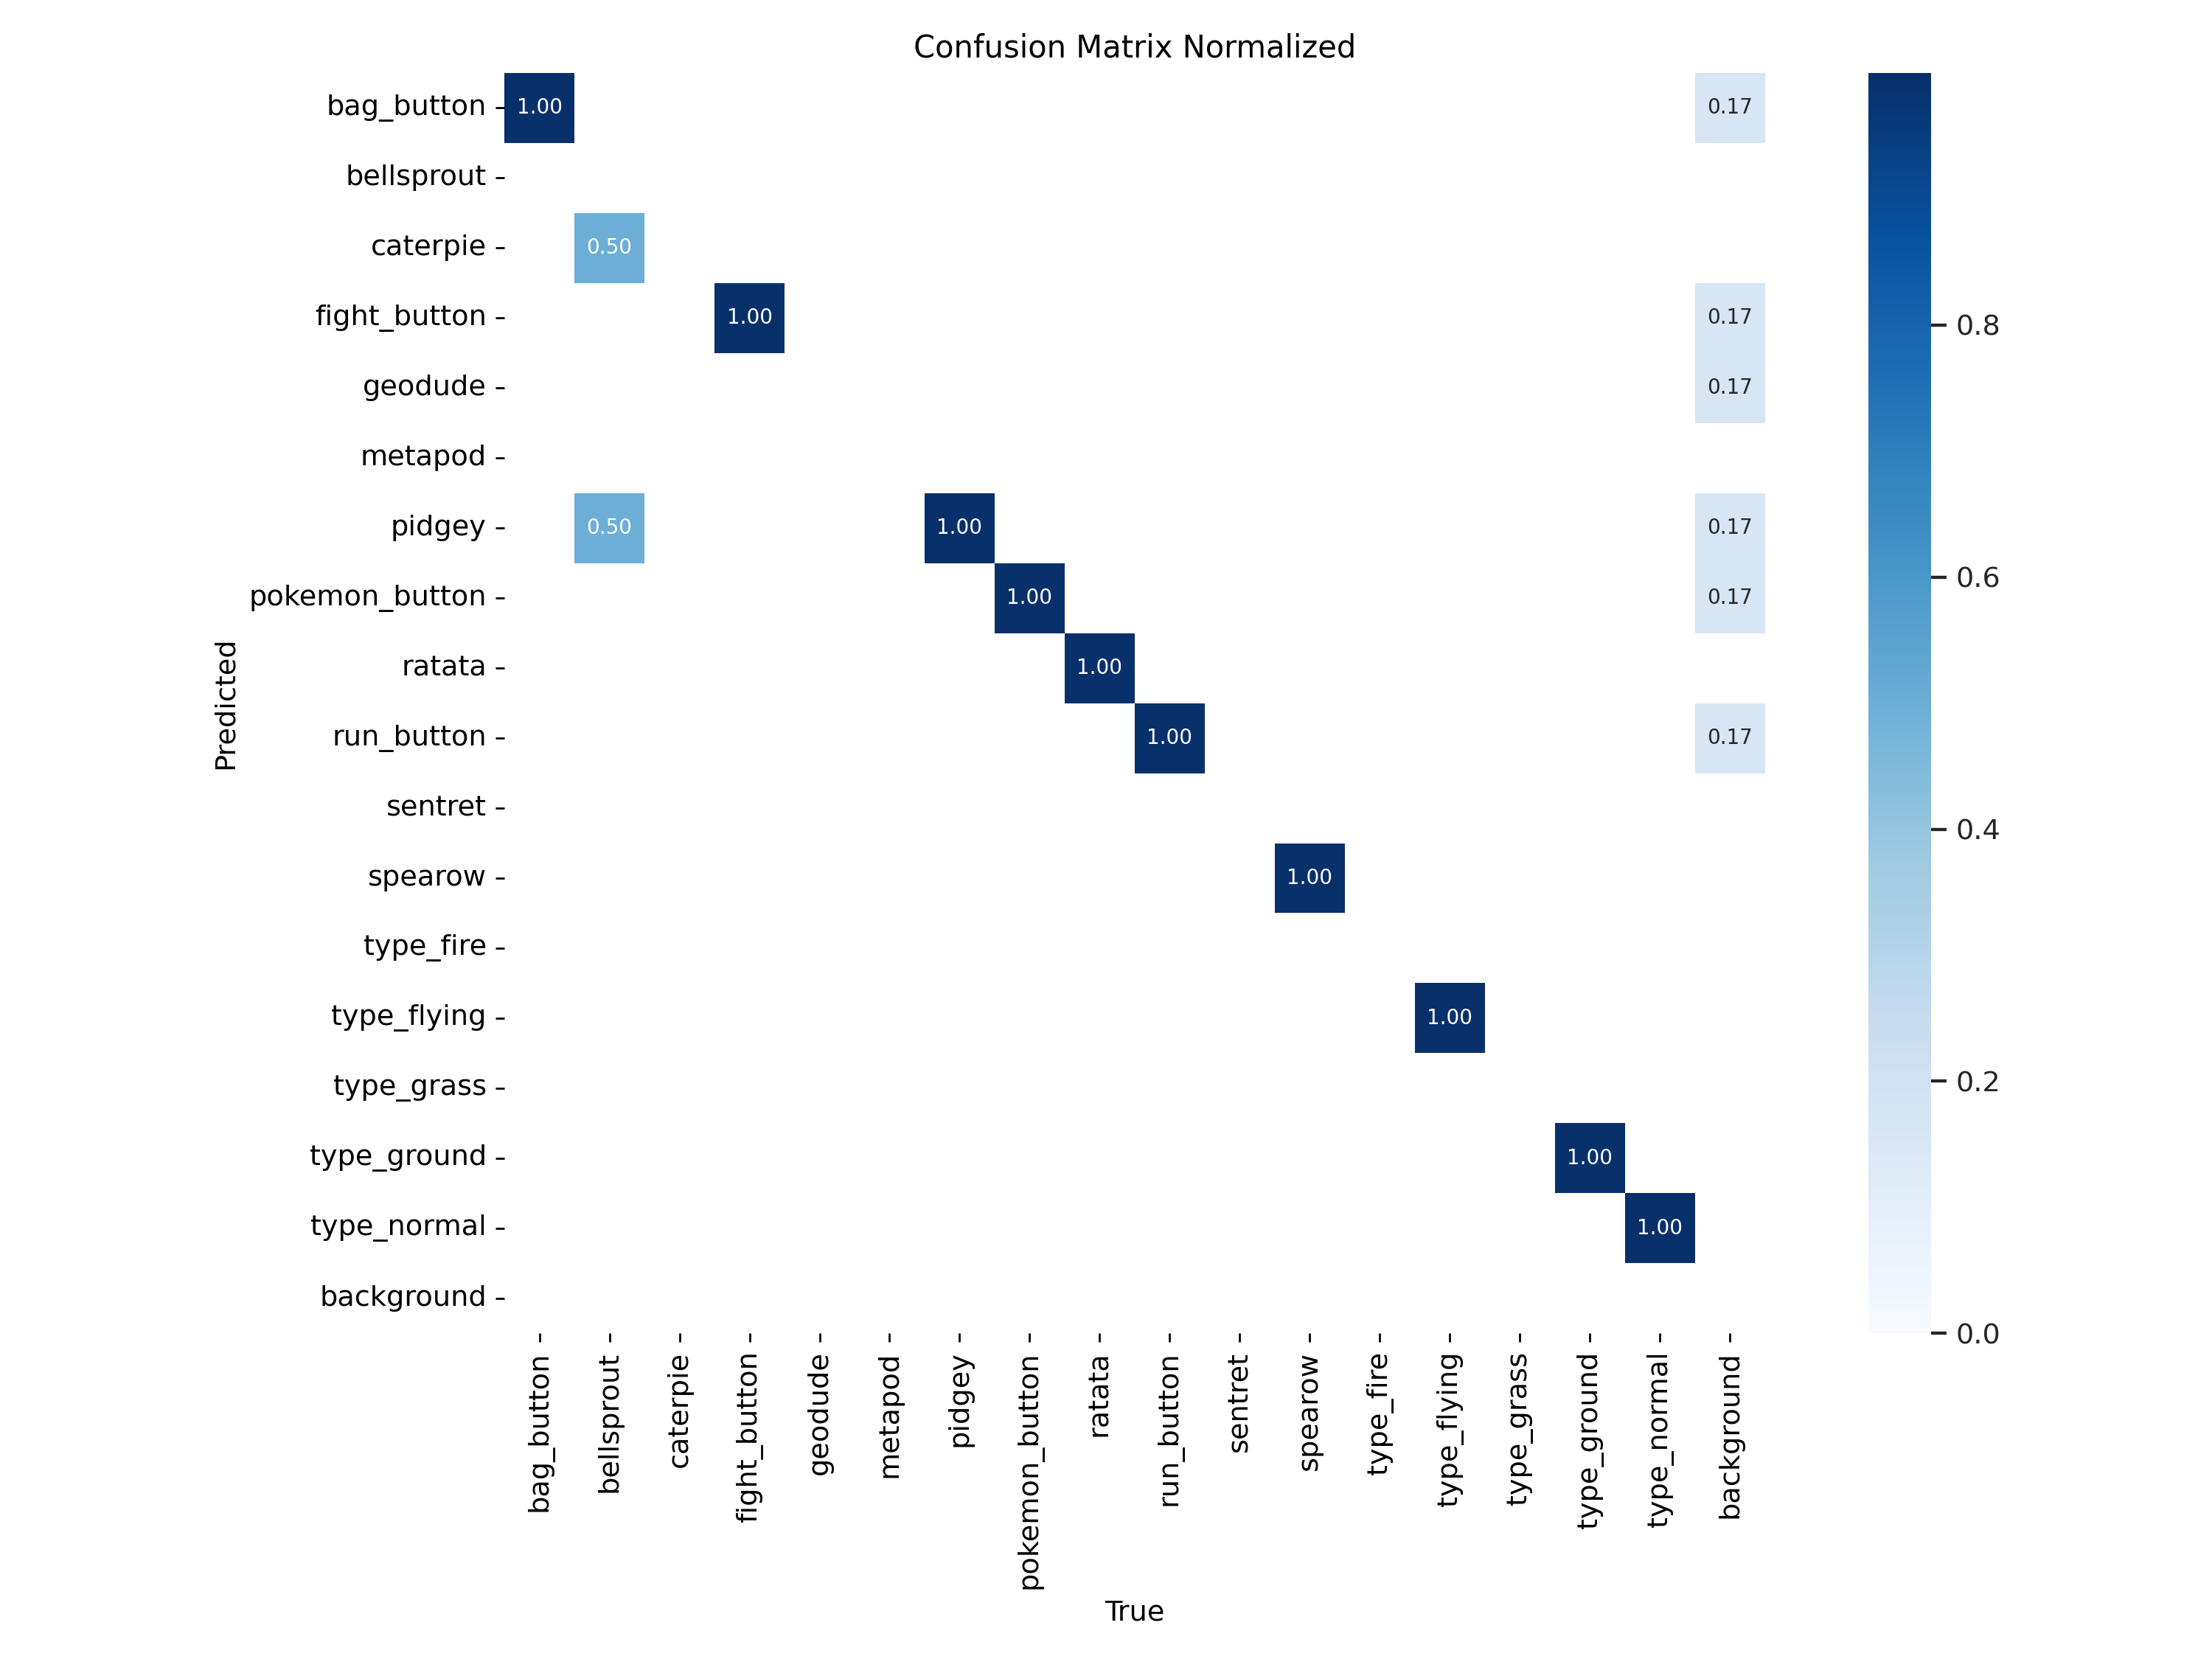
\includegraphics[width=0.65\textwidth]{imagens/confusion_matrix_normalized_primeiro_modelo.png}
    \caption{Matriz de confusão normalizada para o primeiro modelo criado para o Pokémon HeartGold.}
    \label{fig:confusion_matrix_primeiro_modelo}
\end{figure}

\begin{figure}[!h]
    \centering
    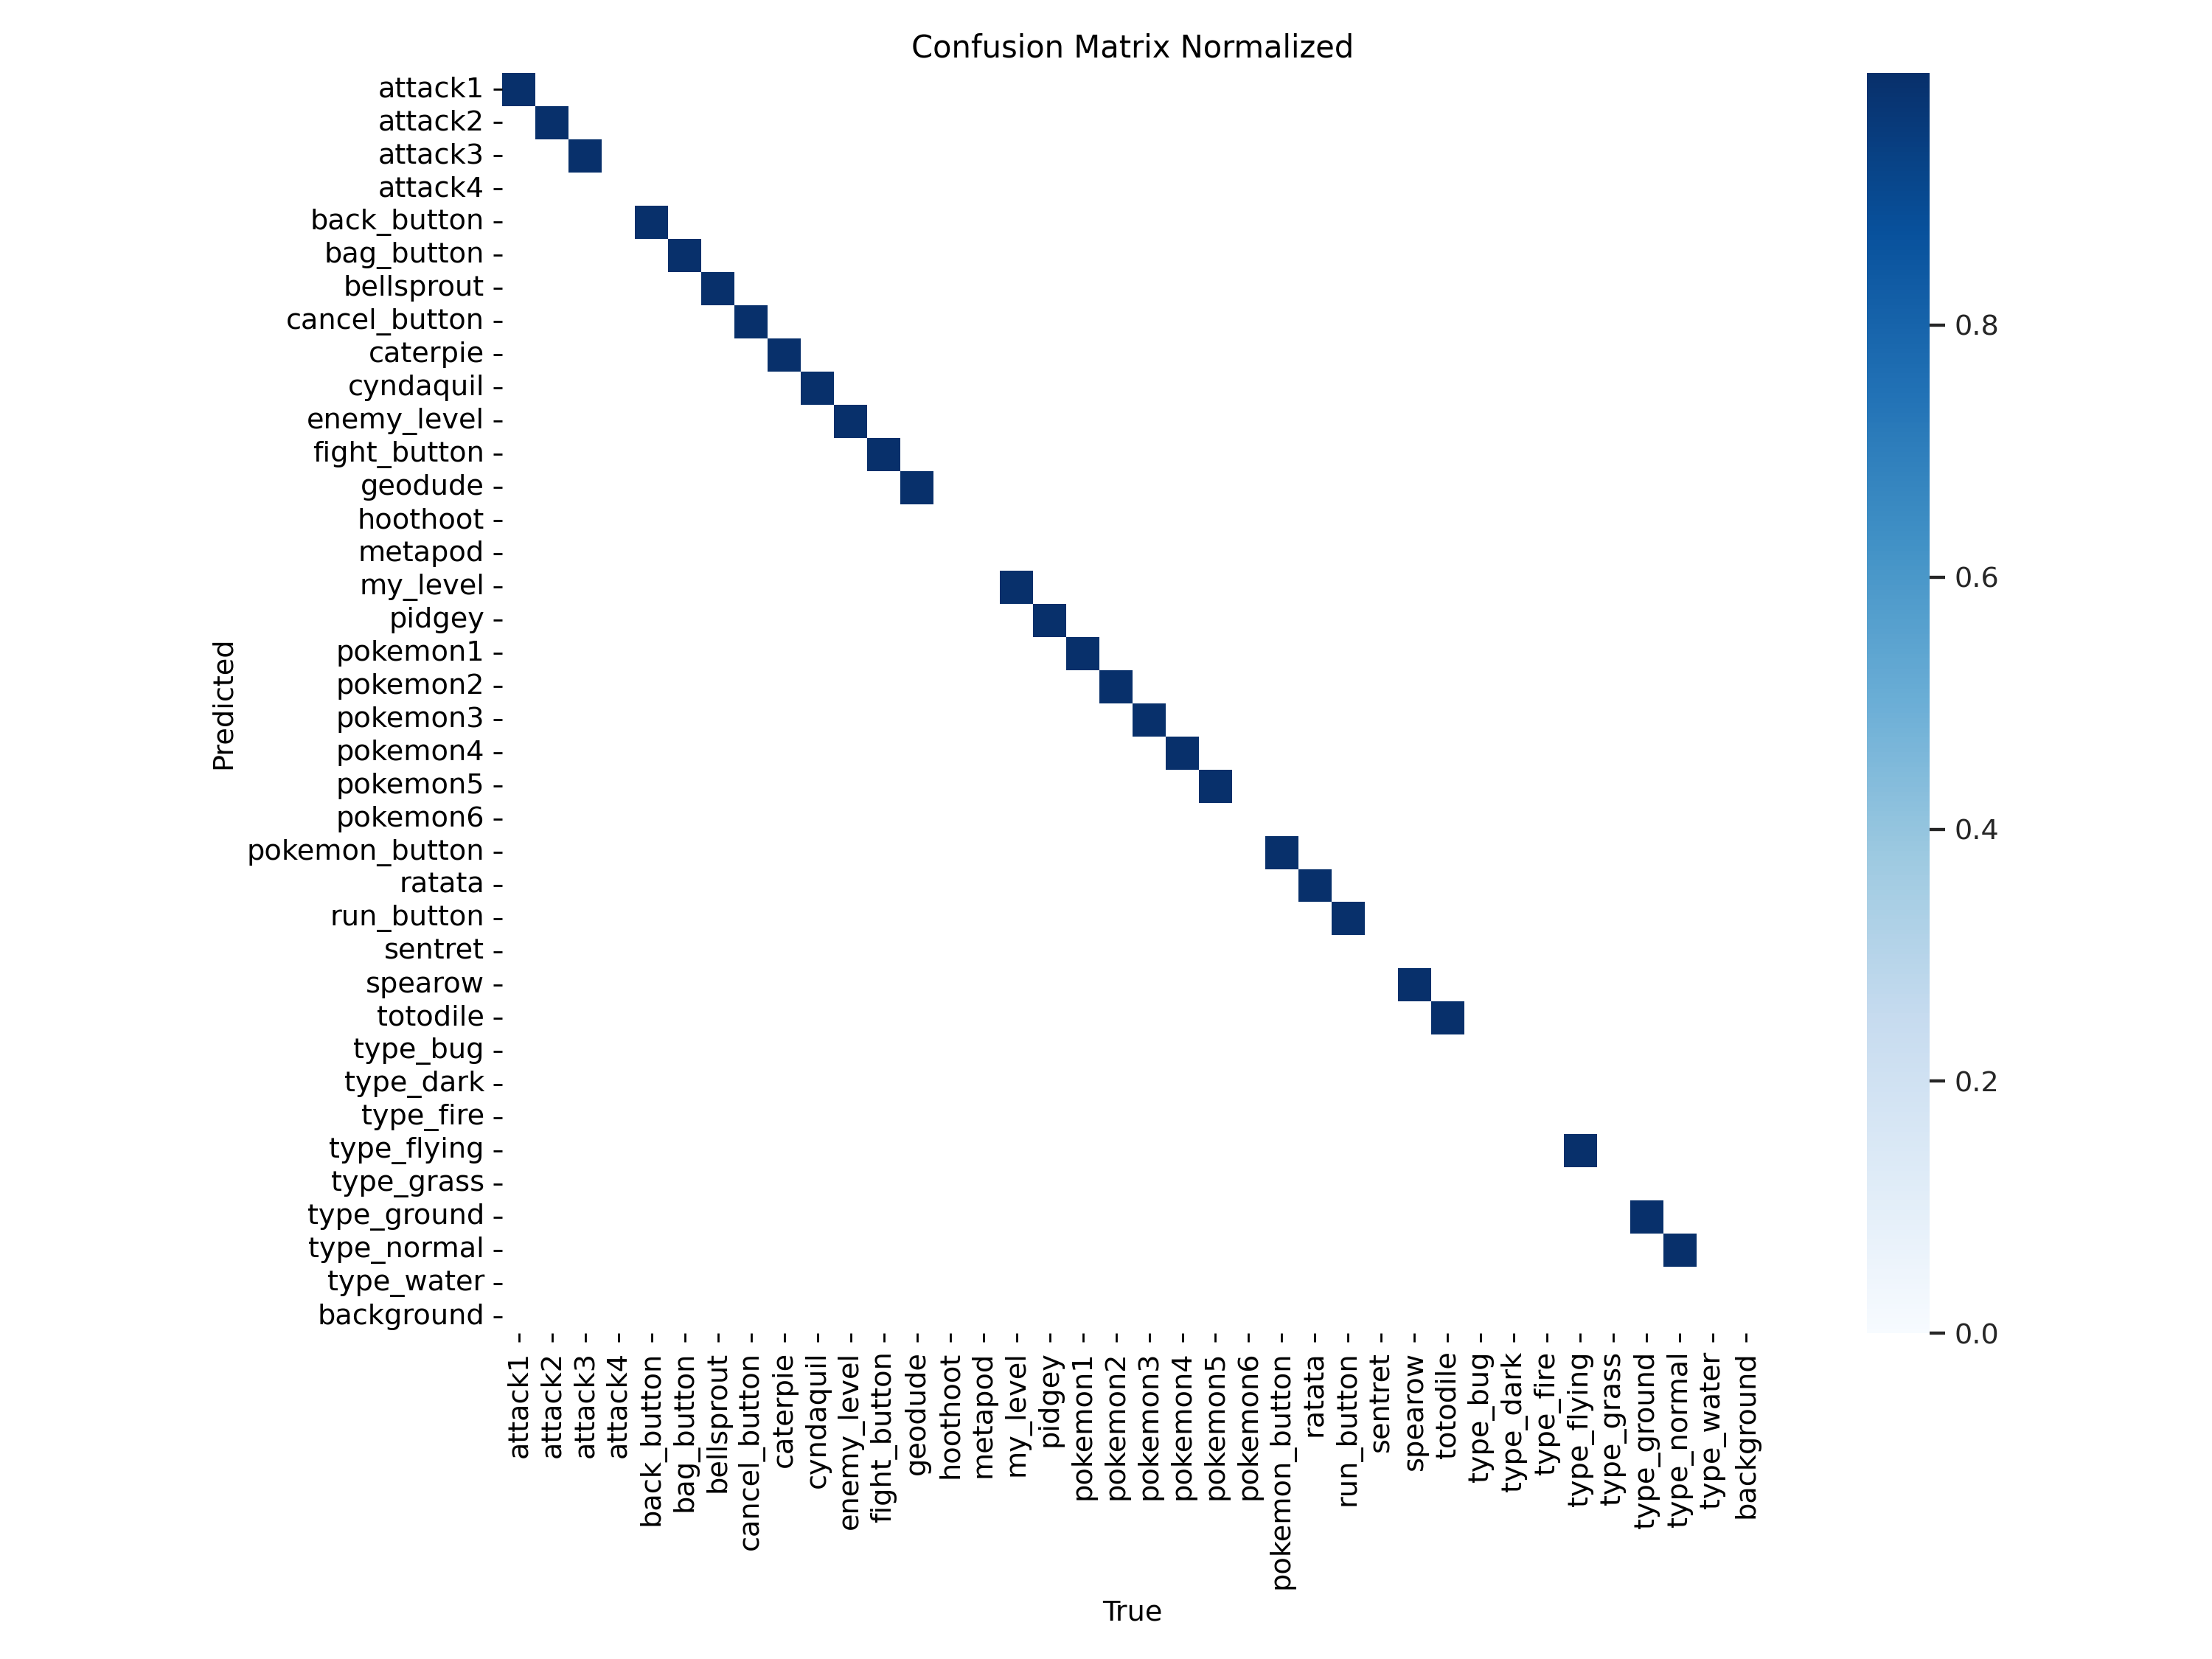
\includegraphics[width=0.80\textwidth]{imagens/confusion_matrix_normalized_segundo_modelo.png}
    \caption{Matriz de confusão normalizada para o último modelo criado para o Pokémon HeartGold.}
    \label{fig:confusion_matrix_ultimmo_modelo}
\end{figure}

Com base na análise das métricas obtidas, observa-se que o segundo modelo apresentou um desempenho significativamente superior, mesmo com um número maior de classes. No entanto, apesar dos resultados quase perfeitos apresentados nas matrizes de confusão normalizadas, é importante interpreta-las com cuidado, pois o facto destas indicarem uma taxa de acerto de 100\% pode não refletir com precisão o desempenho real do modelo em produção. Essa diferença pode estar relacionada com a limitada diversidade do conjunto de validação, possíveis padrões aprendidos especificamente para esse conjunto, ou diferenças nas condições reais de utilização.

Ainda assim, a evolução registada no último modelo em comparação ao primeiro é notável, provavelmente em grande parte devido à aplicação de técnicas de \textit{data augmentation}, que aumentaram a robustez do modelo e a sua capacidade de generalização a novas situações. Assim, justifica-se a escolha deste modelo como versão final para produção.